\subsection{Task 2: phrase table}


A phrase-table can be seen as recursive finite-state transducer that maps contiguous sequences of source words onto contiguous sequences of target words. 
Consider the rules in Figure \ref{fig:table}, the resulting transducer is shown in Figure \ref{fig:rules}. 
Note that the phrase table transducer defines an infinite set of binary relations over $\Sigma^* \times \Delta^*$ (where $\Sigma$ is the source language vocabulary and $\Delta$ is the target language vocabulary).

There are different possible designs and there is not one that is per se a standard.
The one I chose is similar to the one presented in \citep[Figure 6]{Kumar+2003:WFST} and \citep[Figure 1]{Knight+2009:WANLP}.
In my design, there is one initial state which is also final, every translation rule starts and ends in this state.
If a translation rule maps a single source word to a single target word, then this rule can be compactly represented by one arc (see \texttt{black:noir} in Figure \ref{fig:rules}).
Otherwise, when a rule maps $m$ source words to $n$ target words (where $m\neq n$), I decided to first recognise all source words, without producing any target words, and only then to generate target words one by one making sure the last arc of the rule returns to the initial/final state.
Observe that the internal states associated with a certain rule (for example 1, 2 and 3 in Figure \ref{fig:rules}) are there to memorise how much of the rule we have already matched. 
Even though there are more compact ways to represent translation rules, this seems rather clean and easy to turn into an algorithm.


\begin{figure}[h]\centering
\begin{tabular}{l l }
\bf Source & \bf Target \\
\texttt{the} & \texttt{le}  \\
\texttt{the} & \texttt{un} \\
\texttt{dog} & \texttt{chien} \\
\texttt{black} & \texttt{noir} \\
\texttt{black} & \texttt{noirs} \\
\texttt{black dog} & \texttt{chien noir} 
\end{tabular}
\caption{\label{fig:table}Example phrase table.}
\end{figure}


In this task you will have to produce a weighted finite-state transducer for each of the first 100 sentences in \texttt{dev.en}. 
Under \texttt{rules.monotone.dev} you will find one phrase table for each source sentence, they are stored in files named \texttt{grammar.$n$} where \texttt{$n$} is the sequential (0-based) position of the sentence in \texttt{dev.en}.


\begin{figure}[h]\centering
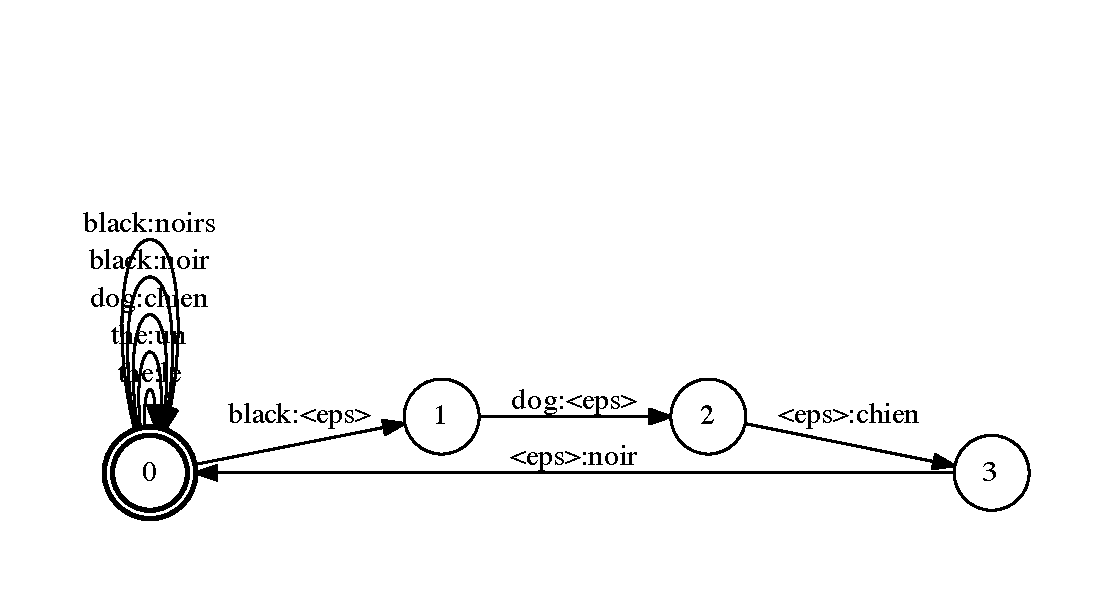
\includegraphics[scale=0.5]{table.pdf}
\caption{\label{fig:rules}Phrase table as a transducer.}
\end{figure}

In a grammar file, each rule is represented by 5 fields separated by 3 vertical bars:

\begin{itemize}
	\item the first field can be ignored
	\item the second field contains the source phrase
	\item the third field contains the target phrase
	\item the fourth field contains a feature map:
		\begin{itemize}
			\item \texttt{IsSingletonF}: whether the source phrase occurred only once in the training data
			\item \texttt{IsSingletonFE}: whether the phrase pair occurred only once in the training data
			\item \texttt{SampleCountF}: frequency of the source phrase in the training data 
			\item \texttt{CountEF}: frequency of the phrase pair in the training data 
			\item \texttt{EgivenFCoherent}: frequency of the target phrase normalised w.r.t. frequency of source phrase
			\item \texttt{MaxLexEgivenF}: lexical smoothing
		\end{itemize}
	\item the last field (which you can ignore) represents the internal alignment of the phrase pair
\end{itemize}

In a phrase-based system, translation rules are parametrised by a linear model.
Let $(f, e)$ be a phrase pair and $\phi: \Sigma^+ \times \Delta^+ \to$ a mapping between phrase pairs and a $d$-dimensional feature vector.
Then each phrase pair $(f,e)$ is associated with a parameter $\theta_{(f,e)} = w^\top \phi(f,e)$ where $w$ is a vector of model parameters.\footnote{In the transducer, you can weight translation rules by weighting one of its arcs, typically the first or the last.}
You will note that rules are annotated with features, those are components in the linear model. You will need those, and the model parameters in \texttt{weights.monotone}, in order to score phrase pairs. 
Besides the features in the phrase table, you need to consider 3 other features which also decompose at the phrase level, but aim mostly at scoring segmentations, namely:
\begin{itemize}
	\item \texttt{Glue}: the total number of phrases used in a derivation - each phrase pair contributes to this feature with a count of $1$
	\item \texttt{WordPenalty}: the total number of target words in a derivation - each phrase pair contributes to this feature with $\frac{-1}{\ln(10)}$ times the number of tokens in the target phrase 
%	\item \texttt{PassThrough}: typically, each unknown source word (a word without an entry in the phrase table) motivates a ``pass-through'' rule, that is, a trivial phrase pair that copies that unknown source word onto the output stream - each such rule contributes to this feature with a count of $1$
\end{itemize}

Finally, to make sure phrase tables can cover all words in the input we typically augment them with ``passthrough rules'' (attention: the phrase tables we provide do not contain such rules, you have to take care of that yourself).
A passthrough rule is a trivial rule that copies a symbol from the input stream onto the output stream. 
%Another way to translate source words which are unknown to the phrase table is to replace them with a special symbol, such as \texttt{Unk}, and add a transition that translates this symbol to itself.
%Whatever strategy you choose, make sure you account for the \texttt{PassThrough} feature when computing the weight of each phrase pair. 
If you watch carefully, you will see that we provided a model parameter for the feature \texttt{PassThrough}.
This feature simply counts the number of passthrough rule applications used in a derivation, in other words, it captures how many source words were unknown. 
Note that as defined, each ``passthrough phrase pair'' contributes to this feature with a count of $1$.
In most cases, this feature is meaningless as the number of unknown source words is constant for each source sentence. 
In practice, for reasons beyond the scope of this section, translation systems might estimate a parameter for this features nevertheless.


\begin{table}[h]\centering
\begin{tabular}{l p{12cm}}
\textsc{Task}   &  encode phrase tables as transducers \\
\textsc{Input}  &  one phrase table per English sentence: \texttt{rules.en-ja.dev.tgz} \\
\textsc{Output} &  one transducers per phrase table in \texttt{rules.en-ja.dev.tgz} \\
\textsc{Submit} &  nothing to submit here\\
\textsc{Report} & discuss the steps involved in creating a phrase table transducer and scoring its arcs, illustrate fragments of phrase tables containing at least one phrase of each of the following types: $1-1$, $m-n$ with $n > m$ and with $m > n$\\
\end{tabular}
\caption{\label{tab:task2}Task 2 summarised}
\end{table}

There are at least two ways do implement passthrough rules:
\begin{enumerate}
	\item  You can add to your phrase table a single translation rule \texttt{OOV:OOV} whose weight is $1\times w_{\texttt{PassThrough}}$, where \texttt{OOV} is a symbol reserved for out-of-vocabulary (OOV) source words. 
Then, you will need to pre-process the source sentence so that every OOV word is replaced by \texttt{OOV}.
For example, if the source sentence is \texttt{the black cat}, then \texttt{cat} is OOV with respect to the phrase table in Figure \ref{fig:table}, we would then pre-process the sentence so that its corresponding transducer recognises/produces \texttt{0:the 1:black 2:OOV}.
\item An alternative method is to pre-process the phrase table as to include rules for each OOV word type essentially making them in-vocabulary. In this case, we would add to our phrase table a rule \texttt{cat:cat} and its score would be $1 \times w_{\texttt{PassThrough}}$. 
\end{enumerate}


Table \ref{tab:task2} summarises the task. 


